\documentclass[11pt]{article}
\usepackage{naacl-hlt}
\usepackage{times}
\usepackage{latexsym}
\usepackage{lingmacros}
\usepackage{graphics}
\setlength\titlebox{6.5cm}    % Expanding the titlebox

\newcommand{\hpsg}{\textsc{hpsg}}
\newcommand{\lkb}{\textsc{lkb}}
\newcommand{\lfg}{\textsc{lfg}}
\newcommand{\itsdb}{\mbox{[incr tsdb()]}}

\newcommand{\mc}{\multicolumn}

\title{Harvesting grammars from the Matrix: Evaluating a bumper crop}
%% \author{Emily M.~Bender, Laurie Poulson, and Scott F. Drellishak\\
%% Department of Linguistics\\
%% University of Washington\\
%% Box 354340\\
%% Seattle, WA 98195-4340, USA\\
%% {\small {\tt \{ebender,lpoulson,sfd@u.washington.edu\}}}
%% \And
%% Dan Flickinger\\
%% CSLI, Stanford University\\
%% Ventura Hall, 220 Panama St\\
%% Stanford, CA 94305, USA\\
%% {\small {\tt danf@csli.stanford.edu}}
%% }

\author{anonymous}
\date{}

\begin{document}
\maketitle
\begin{abstract}
The Grammar Matrix customization system allows users to configure
starter-grammars which add language-specific information across a
range of linguistic phenomena to a cross-linguistic core grammar.
With four phenomenon-libraries implemented so far (word order,
negation, yes-no questions, and coordination) we can already define
hundreds of thousands of language types.  We present a methodology for
creating test suites for any language type generated by the
customization system and then evaluate the current system against those
test suites for a small, random sample of language types.
\end{abstract}

\section{Introduction}

The Grammar Matrix is an open-source starter kit designed to jump-start
the development of broad-coverage precision grammars, capable of both
parsing and generation and suitable for use in a variety of NLP applications.
Initial work on the Matrix ([self-reference omitted])
%Ben:Fli:Oep:02, Fli:Ben:03
focused on the development of a cross-linguistic core grammar.  The
core grammar provides a solid foundation for sustained development of
linguistically-motivated yet computationally tractable grammars (e.g.,
\cite{Hel:Hau:03,Kor:Neu:05}).  However, the core grammar alone cannot
parse and generate sentences: it needs to be specialized with
language-specific information such as the order of daughters in its rules
(e.g., head-subject or subject-head), and it needs a lexicon.
Although word order and many other phenomena vary across languages,
there are still recurring patterns.  To allow reuse of grammar code
across languages and to increase the size of the jump-start provided
by the Matrix, in more recent work ([self-reference omitted]),
%Ben:Fli:05, Dre:Ben:05
we have been developing `libraries' implementing realizations
of various linguistic phenomena.  Through a web interface, grammar
developers can configure an initial starter grammar by filling out
a typological questionnaire about their language, which in turn
calls a CGI script to `compile' a grammar by making appropriate selections
from the libraries.

The initial set of libraries includes: basic word order of major
constituents in matrix clauses (SOV et al), optionality/obligatoriness
of determiners, noun-determiner order, NP v.\ PP arguments of intransitive
and transitive verbs, strategies for expressing sentential
negation and yes-no questions, and strategies for constituent coordination.
Even with this small set of phenomena covered (and limiting ourselves
arbitrarily for testing purposes to a maximum of two coordination strategies
per language), we have already defined a space of hundreds of thousands of possible
grammars.\footnote{If all of the choices in the customization system
were independent, we would have more than 2 x 10$^{27}$ grammars.  In actuality,
constraints on possible combinations of choices (e.g., if a grammar
has two case-marking adpositions, they must both be prepositions or
both be postpositions) limit this space considerably.}

Precision grammar engineering usually proceeds by continually
testing the grammar against hand-constructed test suites as well
as selections from naturally occurring corpora, and refining the
grammar as necessary.  In this case, it is simply not practical to
test all of the hundreds of thousands of grammars.  

Our development methodology has been to test each option in each
library as we create it.  Testing any part of one library involves
instantiating choices from at least a few other libraries (word order,
lexicon).  However, We have not attempted to systematically vary those other
choices (e.g., strategies for expressing
sentential negation may all be tested with SOV grammars).  In this
paper, we describe our methodology for validating the interaction
of the libraries over a random sample of grammars from the 
grammar space and the associated creation of a test suite resource for
future regression testing. 

\section{Background}

The Grammar Matrix is written within the HPSG framework
\cite{Pol:Sag:94,Sag:Was:Ben:03}.  HPSG is a constraint-based grammar
framework implemented in typed feature structures.  HPSG grammars are
declarative resources which can be used by both parsing and generation
algorithms.  The particular variant of the formalism we use is TDL
(type description language) as interpreted by the LKB
\cite{Copestake02} grammar development environment.  The LKB includes
grammar visualizion and debugging tools, a parser, and a generator. 
For test suite management, we use \itsdb\ \cite{Oepen:01}.

The customization system presents users with a
web-based interface through which they may input typological
information about the language they wish to build a grammar for and
then download an appropriately customized version of the Grammar
Matrix.  These little grammars describe very small fragments of the
languages they model, but they are not toys.  Their purpose is to be
good starting points for further development.  Usability
considerations put two important constraints on the customization
system: 

\begin{enumerate}
\item The questions must be ones that are sensible to linguists,
who tend to consider phenomena one at a time.  
\item The output grammar code must be both readable and maintainable.
\end{enumerate}
%
To achieve readable grammar code in the output TDL, among other
things, we follow the guideline that any given constraint is
stated only once.  If multiple types require the same constraint, they
should all inherit from some supertype which bears the constraint.
In addition, all constraints pertaining to a particular type are
stated in one place.

The Grammar Matrix customization system reads in the user's language
specification and then outputs language-specific definitions of types
(rule types, lexical entry types and ancillary structures) which
inherit from types defined in the crosslinguistic core of the Matrix
but add constraints appropriate for the language at hand. The customization
system is implemented as a Python script which builds TDL descriptions,
prints them to the appropriate files, includes the cross-linguistic
shared files, and presents the user with an archive for downloading.

In light of the two basic constraints on the customization system, we
have found that it is not possible to treat the libraries as black-box
modules with respect to each other.  The libraries are interdependent,
and the portions of the script which interpret one part of the input
questionnaire frequently need to make reference to information
elicited by other parts of the questionnaire.  For example, the
customization system implements major constituent word order by
specializing the head-complement and head-subject rule types provided
in the core grammar.  In an SOV language, these would both be
cross-classified with the type head-final, and the head-subject rule
would further be constrained to take only complement-saturated phrases
as its head daughter.  The TDL encoding of these constraints is shown
in Figure~\ref{tdlfig}.

\begin{figure*}[ht]
\small
\begin{center}
\begin{tabular}{l}
\begin{minipage}{5in}
\begin{verbatim}
comp-head-phrase := basic-head-1st-comp-phrase & head-final.
subj-head-phrase := basic-head-subj-phrase & head-final &
  [ HEAD-DTR.SYNSEM.LOCAL.CAT.VAL.COMPS < > ].
\end{verbatim}
\end{minipage}\\
\end{tabular}
\end{center}
\caption{Specialized phrase structure rule types for SOV language}
\label{tdlfig}
\end{figure*}

Following standard practice in HPSG, we use the head-complement phrase
not only for combining verbs with their complements to make VPs, but
also for all other head complement structures, notably PPs, CPs, and
VPs headed by auxiliaries.  These three are notable because they are
all implemented in the Grammar Matrix customization system and
because the order of head and complement can differ among them.
Consider Polish, a free word order language that nonetheless has
prepositions.  The order of a verb with respect to its complements is
free, so we instantiate both head-comp and comp-head rules, which
inherit from head-initial and head-final respectively. Yet the
prepositions must be barred from the head-final version lest the
grammar license {\it post}positional phrases by mistake. We do this by
constraining the {\sc head} value of the comp-head phrase.  Similarly,
question particles (such as {\it est-ce que} in French or {\it ma} in
Mandarin) are treated as complementizers: heads which select for an S
complement.  Since these, too, may differ in their word order
properties from verbs (and prepositions), we need information about
the question particles (elicited with the rest of the information
about yes-no questions) before we have complete information about the
head-complement rule.  Furthermore, it is not simply a question of
adding constraints to existing types: Consider the case of an SOV
language with prepositions and sentence-initial question particles.
This language would need a head-initial head-comp rule that can take
only prepositions and complementizers as its head.  To express the
disjunction, we must use the supertype to {\it prep} and {\it
comp}.  This, in turn, means that we can't decide what constraint to
put on the head value of the head-comp rule until we've considered
questions as well as the basic word order facts.

We expect to study the issue of (non-)modularity as we add additional
libraries to the resource and to investigate whether the grammar code
can be refactored in such a way as to make the libraries into true
modules.  We suspect at this point that while it might be possible to
reduce the degree of interdependence, it will not be possible to
achieve completely independent libaries, because syntactic phenomena
are inherently interdependent. Consider the case of
agreement in NP coordination. In English and many other languages, 
coordinated NPs are always plural, regardless of the number value of the
coordinands.  Furthermore, the person of the coordinated NP is the
minimal person value of the coordinands.  

\eenumsentence{
\item A cat and a dog are/*is chasing a mouse.
\item Kim and I should handle this ourselves.
\item You and Kim should handle this yourselves.}
%
In languages with gender systems, there is often a similar hierarchy
of gender values, e.g., in French coordianted NPs the whole NP is feminine
iff all coordinands are feminine and masculine otherwise.  Thus
it appears that it is not possible to define all of the necessary
constraints on the coordination rules without having access to information
about the agreement system.  

Even if the libraries could be made completely independent at the
customization level, however, the various parts of the grammar need to
be able to interact properly in the analysis of individual sentences.
Any sentence which illustrates sentential negation, a matrix yes-no
question, or coordination also necessarily illustrates at least some
aspects of word order, the presence v.\ absence of determiners and
case-marking adpositions, and the subcategorization of the verb that
heads the sentence.  Furthermore, broad-coverage grammars need to
allow negation, questions, coordination etc.\ all to appear in the
same sentence.

Given the complexity of the system in general and the interdependence
between the libraries, it is not sufficient to test each library in
isolation.  On the other hand, testing all possible combinations is
not computationally tractable.  In practice, in the course of developing
any given library, we define grammars which test all options given
by that library while keeping the rest of the choices more or less constant.
The following sections describe the system we developed for sampling
the rest of the grammar space, providing sentences with associated semantic
representations and well-formedness predictions 
for evaluating any given grammar in that space, and
thereby testing the cross-compatibility of our libraries.

%% Add reference to Poulson 2006 about here.

\section{Remarks on evaluation}

There are many levels at which the Grammar Matrix customization system
could and should be evaluated. At the highest level, its twin purposes
are reducing the cost of developing broad-coverage precision grammars
and crosslinguistic hypothesis testing.  Regarding the first, the
system should be evaluated in terms of how much time and effort it
saves in the development of grammars.  Regarding the second, the
system should be tested against naturally-occuring data as well as
linguist-developed test suites from a typologically balanced sample of
the world's languages.  Each of these evaluations, but especially the
second, is prohibitively expensive.  By using the Grammar Matrix in
grammar engineering courses where students each model different
languages and by soliciting feedback from other users of the system,
we are gathering information from actual languages which, while not
giving any precise measure of the performance or correctness of the
system overall, does allow us to incrementally refine the system.

This paper addresses a logically prior question to evaluation at
the levels of usefulness or correctness, namely, whether the system
indeed performs as intended. Each library is intended to produce
(or play its part in producing) particular semantic representations for
particular types of sentences.  Given the overall complexity of the
system, it is non-trivial to verify whether the libraries each function
as intended.  We describe here how we build the set of reference cases
needed to answer this question, and evaluate the performance of
a system developed with a small set of grammars against a sample
from the much larger set.

In general, with precision grammars, there are three relevant
metrics:

\begin{enumerate}
\item Coverage (\% of grammatical sentences parsed, a type of recall)
\item Overgeneration (\% of ungrammatical sentences parsed, a type of precision)
\item Accuracy (\% exact match on semantics for the sentences parsed)
\end{enumerate}
%
It follows that our gold standard resource will need to include
both 'grammatical' and 'ungrammatical' examples, an indication of the
intended grammaticality of each, and an associated semantic representation.

\section{Methodology}

\subsection{Test suite resource}

In order to test an arbitrary selection from the space of grammars we have
defined, we need a parallel, independent system which can generate a gold
standard for comparison for any abitrary language type.  Fortunately,
this can be a simpler sort of grammar because it can be restricted to a
finite set of sentences.

In creating this test resource, we make two abstractions. The first
concerns vocabulary.  Much of the idiosyncrasy in language resides in
the lexicon, both in the form of morphemes and in the particular
grammatical and collocational constraints associated with them.  While
our customization system allows for some lexical variation (e.g., each
verb can select for either an NP or a PP subject), we assume that
each grammar tested will draw its lexicon from the 
standardized set of lexical entries with standardized forms shown in
Table~\ref{tab1} (though
not all languages will use all of these forms).
Using the same word forms for each grammar contributes substantially
to building a single resource which can be adapted for the testing
of each language type.


\begin{table*}[ht]
\begin{center}
\begin{tabular}{|l|l|l|}
\hline
Form & Description & Options \\ \hline \hline
det & determiner & \\ \hline
n1, n2 & nouns & det is optional, obligatory, impossible\\
tv & transitive verb & subj, obj are NP or PP\\
iv & intransitive verb & subj is NP or PP\\
p-nom, p-acc & case-marking adpositions & preposition or postposition\\
neg & negative element & adverb, prefix, suffix\\
co1, co2 & coordination marks & word, prefix, suffix\\
qpart & question particle & \\
\hline
\end{tabular}
\end{center}
\caption{Standardized lexicon}
\label{tab1}
\end{table*}


The second abstraction has to do with the notions of grammaticality
and language.  The grammars produced by the customization system are
underspecified with respect to actual languages.  For example, they
currently lack any analysis of case (outside the option of
case-marking adpositions) or agreement.  In fact, they will always be
underspecified, no matter how large the system gets, because it is not
possible to describe all of the details of all of the world's
languages in a system like this---just getting the `core' grammar down
will be challenge enough.  Thus one and the same starter grammar might
be extended into multiple models corresponding to multiple actual
human languages.  Accordingly, in what follows, we speak of language
types rather than languages.  When we talk about the predicted
(un)grammaticality of a candidate string, we are referring to its
predicted well- or ill-formedness given the information contained
in the language type definition.

%[INSERT EXAMPLE HERE?]

It turns out it is possible 
%(though not terribly elegant) 
to create a
gold-standard resource by enumerating a set of `seed strings',
producing all possible permutations of them, and then using regular
expressions to filter the permutations.\footnote{This approach is
similar in spirit to \cite{Arnold*94}.}  
%This process is schematized
%in Figure~\ref{filter_fig}.

The seed strings can be grouped into semantic equivalence classes.
From each equivalence class, we select one representative string which
we parse with an appropriate grammar derived from the Matrix
customization system.  The parses that the LKB returns are actually
large feature structures.  From the feature structure, we `harvest' the
sub-feature structure which encodes the semantic representation of the
whole string.

The remaining seed strings in the equivalence class differ from each
other and from the `harvester' string in the presence or absence of
various semantically empty elements (case-marking adpositions and
tense-marking auxiliaries\footnote{The auxiliaries are only
semantically empty currently because we don't yet have an analysis of
tense/aspect.})  and the affix v.\ word status of some of the
formatives (negation, coordinator).  To get the full set of candidate
strings for a given semantic representation, we take all permutations
of the formatives (including affixes) in each seed string.
%TODO: Put in figure showing how set of strings grows.

The strings are filtered in two passes---once to remove strings which
are predicted to be ungrammatical in all language types and a second time
relative to the particular langauge type being tested.  On each
pass, a selection of ungrammatical examples is retained (and marked as such)
in order to test for overgeneration.  It is not practical to retain
all ungrammatical examples, as the resulting test suites would be too
large (millions of sentences).

The filters are sensitive to the intended semantics of the candidate
strings.  This is important for two reasons: First and foremost, it
allows us to create a resource against which to measure the accuracy
of the grammars, that is, their ability to produce all and only the
correct semantic representations for a particular string.  In many
cases, the same string might well be grammatical in different language
types, but only on different interpretations.  For example, in a VSO
langauge, {\it tv det n1 det n2} would be mapped to a declarative
representation with `n1' as the first semantic argument.  In a VOS
language, the same string would be mapped to a declarative
representation with `n2' as the first semantic argument.  And in an
SVO language which expressed yes-no questions with subject-verb
agreement, that same string would map to a question representation
with `n1' as the first semantic argument.

Second, giving the filters access to semantic representations allows
us to write filters for each dimension of variation mostly
independently from the other dimensions.  For example, since we know
that the candidate strings with the same semantics as {\it det n1 det
n2 tv} all have exactly two determiners in them, we can check that the
determiners are adjacent to the nouns with the regular expression in
(\ref{re1}).

\enumsentence{\label{re1}
{\tt\small det n[12].*det n[12] $\mid$ det n[12].*n[12] det $\mid$ n[12] det.*n[12] det $\mid$ n[12] det.*det n[12]}
}
%
Because we know, for any given equivalence class, what words might be
in the string, it is easier to write filters that only make reference
to one or two properties of the language definition at a time. This,
in turn, means that we can create a gold standard resource over our
particular seed strings for any language type that can be generated by
the system.

A further complication arises in the case of ambiguous harvester
strings.  In our current set of seed strings, this arises with
the coordination examples.  The example in (\ref{co1}) has two
semantic representations, schematized in (\ref{co2}).

\enumsentence{\label{co1}
det n1 co1 n1 co1 n1 iv (cf.\ The horse and buggy and wagon left)
}

\eenumsentence{\label{co2}
\item iv (and (n1, and (n1, n1)))
\item iv (and (and (n1, n1), n1))
}
%
To handle this, we generalize the string-semantic representation mapping
to relate strings to sets of semantic representations.  In most cases,
our candidate strings have just one semantic representation.  In the
ambiguous cases, they have more than one.  The process of permuting
the formatives of the seed strings can create candidate string-representation
pairs with the same string.  When we have created the gold-standard resource
for a particular language type, we search for such cases and collapse them
into one entry, where all of the semantic representations are included in
its set.

In summary, candidate strings mapping to the same semantics can vary
in the lexical elements they contain or the order of the lexical
elements.  We handle the first by enumerating seed strings and the
second by permuting the lexical elements.  The process of associating
seed strings to semantic representations, creating candidate
string-representation pairs, and then filtering them is shown in
Figure~\ref{filter_fig}.

\begin{figure}[ht]
\begin{center}
\scalebox{.5}{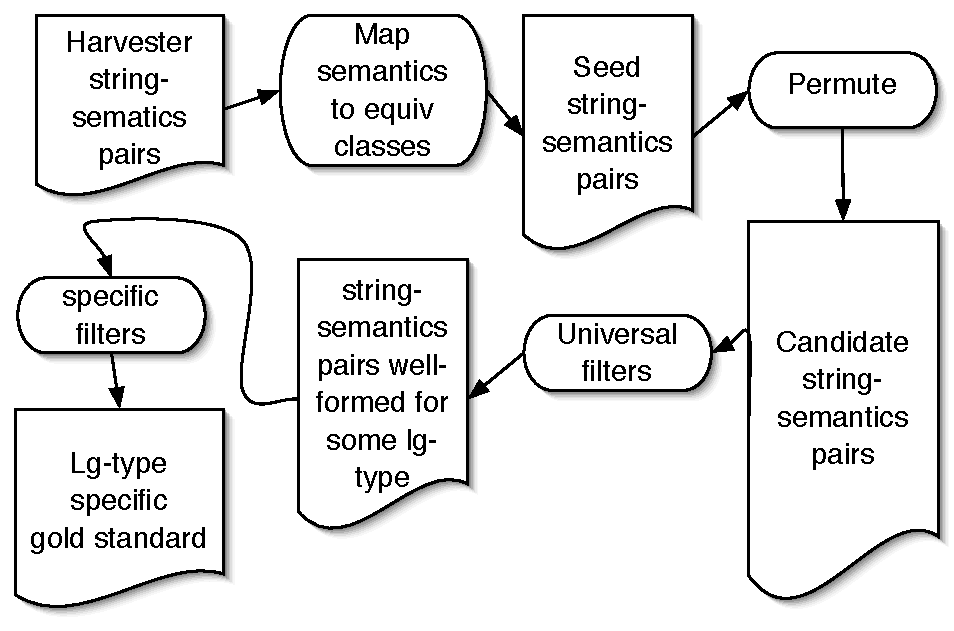
\includegraphics{strings}}
\end{center}
\caption{Filtering process}
\label{filter_fig}
\end{figure}

\subsection{Random grammars}

Underlying both the customization script and the web-based
questionnaire form is a single file which defines the parameters
available for configuration, their possible values, and how the choice
should be displayed in the web interface presented to the user. We
take advantage of this file yet again in a third script which reads it
in and produces randomly selected grammars.  For each choice it randomly
selects among the possibilities (including the possibility of making
no choice at all).  The result is then run through the same validation
routine that we use on the web page to alert users if they've made
incompatible or incomplete specifications.  Only grammars that pass
the validation constraints are used.

\section{Results}

\subsection{Test grammars}

We worked with roughly 20 hand-configured grammars in developing the
filters.  In addition, we used 15 randomly generated grammars 
to do further debugging.  We then produced 4 more randomly
generated grammars and used them to measure system performance. Note
that we are comparing the output of two separate systems (the grammars
and the filters), and points of disagreement can indicate an error
on either side.  This is explored further in \S\ref{error}.

\subsection{Performance}

%%%%%%%%%%%%%%%%%%%%%%%%%%%%%%%%%%%%%%%%%%%%
%%                   Non-coord  Coord   Total
%% Harvest           18         12      30
%% Other seed        124        84      208
%% Candidates        9711188    3043584 12754772

Our 30 harvester strings and 208 other seed strings together produced
12,754,772 candidate string-semantics pairs.  
% Previous number includes lots of duplicates.  Fix that for final
% version. Number belows don't include coordination.
Of these pairs, 25,840 were deemed
potentially grammatical in some language.  258 universally
ungrammatical examples (up to four per seed string) were kept.  This
universal resource was used as the input for creating the language
type-specific resources for 3 language types.  In addition to the
selection of universally ungrammatical examples, a selection of
examples that would otherwise have been filtered at the language-type
specific level was also kept.  The test suites for our test language
types are described in Table~\ref{tab2}.

\begin{table}
\begin{tabular}{|r|r|r|r|r|}
\hline
Lg.~type & Gram. & \mc{1}{|c|}{Avg.} & Ungram & Total\\ 
& & readings & & \\ \hline\hline
1. & 38 & 1.23 & 358  & 396\\ \hline
2. & 3 & 1 & 342 & 345\\ \hline
3. & 6 & 1 & 377 & 383\\ \hline
\end{tabular}
\caption{Language-specific test suites\\
(Preliminary numbers)}
\label{tab2}
\end{table}

For each language type, we calculated coverage (\% of grammatical
strings which parsed), overgeneration (\% of ungrammatical strings
which parsed), and semantic accuracy (\% of test items for which we
have exactly the right set of readings).  The results are shown in
Table~\ref{tab3}.

\begin{table}
\begin{tabular}{|r|r|r|r|r|r|}
\hline
Lg.~type & \mc{2}{|c|}{Coverage} & 
\mc{2}{|c|}{Over-} & {Accuracy}\\ 
& \mc{2}{|c|}{} & \mc{2}{|c|}{generation} & \\ \hline
& \# & \% & \# & \% & \%\\ \hline\hline
1. & 26 & 68.4 & 3 & 1.6 & 63\\ \hline %# 032
2. & 3 &  100 & 2 & 0.6 & 100\\ \hline %# 031
3. & 2 & 33.3 & 2 & 0.5 &  33\\ \hline %# 035
\end{tabular}
\caption{Performance of test grammars\\
(Preliminary numbers)}
\label{tab3}
\end{table}

\subsection{Error analysis}
\label{error}

The errors (both under- and over-generation) in Grammar 3 all relate
to a single bug in the customization script.  In this language, n1 has
an obligatory specifier while n2 can't take a specifier at all.  The
customization script is erroneously making the specifier obligatory
for all nouns. A related problem leads to the overgeneration in Grammar 1.

Grammar 1 is a particularly interesting case.  It has more positive
test items than the rest because it is a free word-order type.  The
ungrammatical examples are all clustered in the negation seed strings.
This language type has specified VP attachment of the negative adverb as
the means of expressing sentential negation.  However, in some of the
possible orders of S, V, and O, there is no VP, that is, no constituent
which combines the V and O to the exclusion of S.  Thus, there is nowhere
for the VP-modifying adverb to attach.  In this situation, the filters
do not match what we have coded in the grammar customization system, and
indeed, it is not entirely clear how to interpret this combination of
choices.  

\section{Conclusion and future work}

This initial system has allowed us to validate the testing approach
and evaluate the grammar compilation system.  It has also proved
itself handy in diagnosing bugs in the compilation code, and we
expect to be able to report on the effect that considering a larger
sample of grammars in the debugging phase has on the performance
of grammars sampled for testing.  While the system is quite complex,
we expect a moderate amount of further refinement to iron out most
of the bugs.

We envision extending the current system by adding seed strings which
more extensively test the interaction between the various modules
(e.g., negation, questions, and coordination all in one), as well as
more thorough coverage of the coordination module.  More importantly,
we are actively working on extending the linguistic coverage of the
libraries provided in the customization system.  As we do so, the
verified test suites discussed here provide a baseline for regression
testing.  Furthermore, as the error analysis above suggests, we expect
the bulk of the cases of filter-grammar mismatch to appear in
typologically unusual grammar specifications.  Thus, this test suite
resource will also aid us in exploring the typological predictions of
our system.

\bibliographystyle{acl}
\bibliography{masterbib}


\section*{A. Appendix}

The following strings were parsed with an SOV grammar with
optional determiners in order to get the semantic representations
for their equivalence class.  Each string is paired here with an English
example where n1 is {\it cats}, n2 is {\it dogs}, and the verbs
as {\it slept} and {\it chased}.  Note that, while a number of the
coordination examples at the end share the same English gloss, their
strings all differ and represent some of the many attested marking
strategies for coordination.  In our analysis, these strategies differ
subtly in their semantics, including their degree of ambiguity (cf.~[self
reference omitted]).
%Dre:Ben:05

\hspace{-15pt}
\begin{tabular}{ll}
n1 iv & cats slept\\
det n1 iv & the cats slept \\
n1 n2 tv & cats chase dogs\\
det n1 det n2 tv & the cats chase the dogs\\
det n1 n2 tv & the cats chase dogs\\
n1 det n2 tv & cats chase the dogs\\
n2 n1 tv & dogs chase cats\\
det n2 det n1 tv & the dogs chase the cats\\
det n2 n1 tv & the dogs chase cats\\
n2 det n1 tv & dogs chase the cats\\
n1 n2 neg tv & cats don't chase dogs\\
det n1 det n2 neg tv & the cats don't chase \\
 & \phantom{...}the dogs\\
n2 n1 neg tv & dogs don't chase cats\\
det n2 det n1 neg tv & the dogs don't chase \\
 & \phantom{...}the cats\\
n1 n2 tv qpart & do cats chase dogs?\\
det n1 det n2 tv qpart & do the cats chase the dogs?\\
n2 n1 tv qpart & do dogs chase cats?\\
det n2 det n1 tv qpart & do the dogs chase the cats?\\
det n1 n1 co1 n1 iv & the cats, cats, and cats slept\\
\end{tabular}
\begin{tabular}{ll}
det co1 n1 co1 n1 co1 & \\
\phantom{...}n1 iv & the cats, cats, and cats slept\\
det n1 co1 n1 co1 n1 iv & the cats, cats, and cats slept\\
n1 n1 co1 n1 iv & cats, cats, and cats slept\\
co1 n1 co1 n1 co1 n1 iv & cats, cats, and cats slept\\
n1 co1 n1 co1 n1 iv & cats, cats, and cats slept\\
det n1 n1 co2 n1 iv & the cats, cats, and cats slept\\
det co2 n1 co2 n1 co2 & \\
\phantom{...}n1 iv & the cats, cats, and cats slept\\
det n1 co2 n1 co2 n1 iv & the cats, cats, and cats slept\\
n1 n1 co2 n1 iv & cats, cats, and cats slept\\
co2 n1 co2 n1 co2 n1 iv & cats, cats, and cats slept\\
n1 co2 n1 co2 n1 iv & cats, cats, and cats slept\\
\end{tabular}



\end{document}

